% Journal:
%   Journal of Ambient Intelligence and Smart Environments (JAISE), IOS Press
%   Web Intelligence and Agent Systems: An International Journal (wias)
% Latex 2e
% Test file iosart2c.tex

%[seceqn,secfloat,secthm,crcready]

% options: wias, jaise
\documentclass{iosart2c}


\usepackage[T1]{fontenc}
\usepackage{times}%

%\usepackage{natbib}
\usepackage[numbers]{natbib}

%\usepackage[dvips]{hyperref}
\usepackage{amsmath}
\usepackage{dcolumn}
%\usepackage{endnotes}
\usepackage{graphics}


%========================== MY PACKAGES ================================%

%pseudocode
\usepackage{algorithm}
\usepackage{algpseudocode}

%draw artificial neural networks
\usepackage{neuralnetwork}
\usepackage{xpatch}
\makeatletter
\xpatchcmd{\linklayers}{\nn@lastnode}{\lastnode}{}{}
\xpatchcmd{\linklayers}{\nn@thisnode}{\thisnode}{}{}
\makeatother

%figures
\usepackage{graphicx}
\usepackage{graphics}
\usepackage{caption}
\usepackage{subcaption} %subimagenes

%math
\usepackage{amsmath,amssymb,amsfonts,amsthm} %for mathematics fonts 
\usepackage{stmaryrd}

%For ORCID logo
\usepackage{svg}


%========================== MY PACKAGES ================================%




\newcolumntype{d}[1]{D{.}{.}{#1}}


\firstpage{1} \lastpage{5} \volume{1} \pubyear{2009}


\begin{document}
\begin{frontmatter}                           % The preamble begins here.

%
%\pretitle{Pretitle}
\title{Evolving neural networks for threat process detection using autoencoder to build a fitness function.\thanks{Footnote in title.}}

\runningtitle{Evolving neural networks for threat process detection using autoencoder to build a fitness function.}
%\subtitle{Subtitle}


\author[A]{\fnms{Henry D.} \snm{Navarro H.}\thanks{Corresponding author. E-mail: contact@henrynavarro.org.}\thanks{Do not use capitals for the author's surname.}},
\author[B]{\fnms{Héctor} \snm{Bullejos}}
and
\author[B]{\fnms{Carmelo} \snm{Garrido}}
and
\author[B]{\fnms{Elena} \snm{Naranjo}}
\runningauthor{H. Navarro et al.}
\address[A]{Research and Development Lab, Vision Analytics, Avenida de Europa 19, 28224, Pozuelo de Alarcón, Madrid,\\ Spain\\
E-mail: contact@henrynavarro.org}
\address[B]{Research and Development Labs, Capgemini Engineering, Calle Campezo, 1, 28022, Madrid, Spain.\\
E-mail: engineering@capgemini.com}

\begin{abstract}
Threat detection is one of the main focus of several studies in the cybersecurity area and it has become one of the main focuses of researchars. Threat may occur in any forms like viruses or phishing attack with different purposes. Once the intruder has filtered into our system, the primary step is to try to detect the malicious process to prevent it from causing damage to our system. In this paper, we present a hybrid method using deep neural networks to obtain a fitness function and evolutionary algorithms to detect and kill malicious processes on a simulated network system in streaming.
\end{abstract}

\begin{keyword}
Neuroevolution \sep Genetic Algorithms \sep Threat detection \sep Autoencoders
\end{keyword}

\end{frontmatter}



\section{Introduction}

Cybersecurity has become into one of the main topics of the last years due to...\\

In order to simulate a network, attack computers with a malicious process and having an environment under control, we have created a virtual network with 20 virtual instances using open source softwares. We start from the fact that the malicious process has infiltrated in our system either using ransomware, social engineering or any other common technique in modern cybersecurity. We collect the system data of these virtual instances using open source libraries. This data will be used to train neural networks, and detect and kill the malicious process using evolutionary algorithms.\\

Evolve neural networks has been used in different tasks but mainly in train neural networks to play video games \cite{deepGA}, \cite{neuroevolution1}, \cite{neuroevolution2}, although there are other applications as music generation \cite{neuroevolution3} and modelling biological phenomena \cite{neuroevolution4}. These neural network training methods rely on genetic algorithm operations to obtain the best agent to perform a specific task. However, there is no too much research related with this topic and cybersecurity as we will see in the section \ref{relatedwork}.\\

Any evolutionary algorithm needs a fitness function in order to determine what agents or individuals are the best in each generation. In our case, the best agents will be those who ``kill'' the malicious process in each generation which will result in instances which take their ``normal states''. In order to characterize this normal state, we use an ingenuous solution for this need, using an artificial neural network called autoencoder. This neural network will learn the healthy state of each instance and using the mean square error (MSE) between the inputs and outputs of the neural networks, we will know how infected is the instance, so the more close this value to zero the more healthy is the state of the instance, so we will use the better agents following this criteria. Then, using the simple command of any Linux system has, we kill the process who is negatively affecting our virtual instance.


\section{Related work}\label{relatedwork}

Autoencoders are neural networks that consist of an encoder to generate a vector of features in the latent space (of smaller dimension) and from the input data and a decoder, which seeks to reconstruct the input data from this latent vector \cite{autoencoders_nlp1}. This type of neural network is used in anomaly detection \cite{anomaly1, anomaly3},\cite{anomaly4}, natural language processing \cite{autoencoders_nlp1} and dimensionality reduction \cite{dimred1}, \cite{dimred2}.\\

Others researchers have proved that autoencoders can be used to detect attacks as Denial of Services \cite{autoencoderdos}. In their paper, \citeauthor{autoencoderdos}, they use an autoencoder to classify different denial of services attacks. However, our objective is not only to classify the state of a virtual machine between two states: healthy and under attack but, to get a measure to quantify how infected an virtual instance is. For this, we train this neural network just with the healthy state data and we will use the mean square error (MSE) as a fitness function to choose the best agents in threat detection, the more close this value to zero the more healthy is the state of the instance.\\

As for the topic of deep neuroevolution, there is no direct application in the area of cybersecurity. However, other researchers have applied genetic algorithms to improve network security \cite{GA1, GA2, GA3}. In most of these papers, a binary gene is reached out in order to block or detect certain networks attacks as Syn-Flood, Smurf and others, for this purpose, common operations in genetic algorithms as selection, crossover, mutation are used.\\

Different investigations in malware detection have been carried out using deep neural networks for them \cite{malwarednn1, malwarednn2,malwarednn3}, however, these researchers train their models using algorithms that involve gradients. In this paper, we present other way to train a neural network that can detect a malicious process that create idle tasks that affects common system values like CPU, memory RAM, hard drive, etc. This process is detected and killed in order to return the healthy state in a virtual instance.

\section{Methodology}

\subsection{Network simulation}

The virtual network to emulate the attacks was built and simulated based on the fact that an intruder had already obtained access to the network and already represents an internal threat, that is, the file that executes the malicious process is already found in the virtual instances. In the figure \ref{fig:virtual_network} we saw an architecture of our virtualized network where we have 20 instances using an a network orchestrator with 4 physical machines.\\


\begin{figure}[h!]
\centering
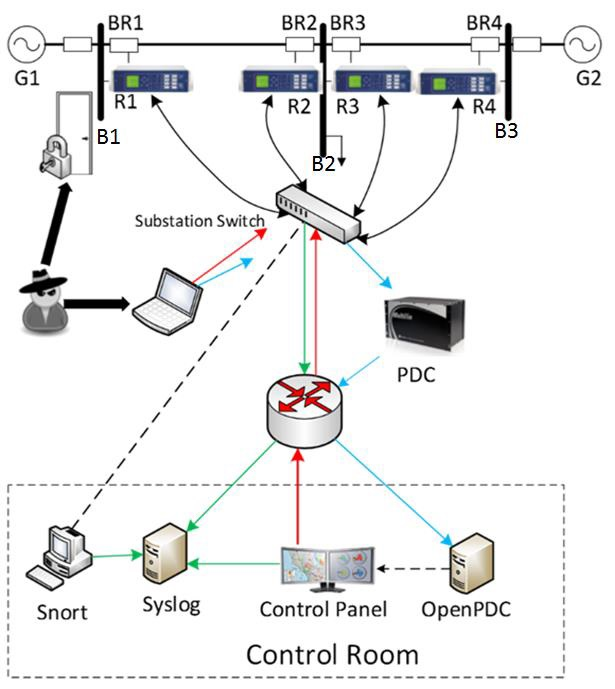
\includegraphics[scale=0.56]{figs/network/diagrama_ejemplo.jpg}
\caption{\textbf{ESTA NO ES LA IMAGEN, AQUÍ TIENE QUE IR UNA IMAGEN DE LA RED, TENGO QUE PEDIRLE AYUDA A FERNANDO A VER SI TIENE TIEMPO.}}
\label{fig:virtual_network}
\end{figure}

These instances send their system data to a NoSQL database where we monitorize the variables that we explain in the next section and these are the features we use to develop our models.

\subsection{Dataset}\label{dataset_autoencoder}

The dataset has been generated first extracting the normal traffic of a virtualized environment to get the ``healthy'' data that a system could have, to get this normal behaviour we used a software tool able to extract 97 features related mainly with cpu, memory ram or usage of hard drive that we split into 10 main groups. Then, the two cyber attacks have been sent to this virtualized network and extracting the data to obtain two new classes: A malicious process developed by us that we will call \textit{Logic Bomb}, which is a process that affects the regular parameters like CPU, memory, disk creating idle processes by this task.

\subsubsection{Central Processing Unit (CPU) features}
They refer to the load characteristics that the CPU of the instance may have. A malicious process acting on the instances is expected to drive CPU usage across the entire instance in order to crash it.\\


\subsubsection{Core features}

These features are similar to CPU variables, with the difference that they are disaggregated by core. Due to how virtualized instances have been created (1GB of memory, 1 core only), these variables are expected to have a high correlation with those of the CPU.


\subsubsection{Disk Input/Output (Disk I/O) features}

Disk I / O operations include both read and write or Input / Output (usually defined in KB / s) involving a physical disk. In simple words, it is the speed with which the data transfer takes place between the hard disk drive and RAM, or basically it measures the input / output time of the active disk. It is a performance measure and is therefore used to characterize storage disks as HDD, SSD, and SAN. A malicious process is expected to constantly perform read and write operations to cause a saturation of this hardware. \\

\subsubsection{Entropy}
Entropy available on the system.

\subsubsection{Filesystem}

This set of features refer to file system statistics on disk. Some malicious processes create an infinite loop that creates files indefinitely in order to saturate it. \\

\subsubsection{Memory Swap}

When the physical memory or RAM in our system is full, we proceed to use the \textit{Memory Swap} in our systems. In this process, the inactive pages of our memory are moved to the swap space, creating more memory resources. This space is especially useful when a system does not have RAM; however, the swap space is located on the hard drive and is therefore slower to access. Therefore it should not be considered as an alternative to RAM. As indicated above, a malicious process is expected to crash RAM memory and from there, begin to consume the resources of swap memory.


\subsubsection{Memory hugepages}

Hugepages are useful in managing virtual memory on Linux systems. As the name implies, they help manage large pages in memory that are larger than the default (usually 4KB). Hugepages is useful for both 32-bit and 64-bit configurations. Hugepages sizes can range from 2MB to 256MB, depending on the kernel version and hardware architecture. A malicious process is expected to increase the values of this variable. \\



\subsubsection{Socket summary}
These variables refer to the summary of open socket metrics in the system. A socket is nothing more than a communication channel between two programs that run on different computers or even on the same computer. Malicious processes seeking to attack the network are expected to affect these variables.  \\


\section{Anomaly detection classification for fitness function}\label{autoencoder_section}

An autoencoder neural network is an unsupervised learning algorithm that applies backpropagation, configuring the target values to be equal to the inputs. That is, the response variable that the machine learning algorithm tries to learn is such that $y^{(i)} = x^{(i)} $, where $x^{(i)} = \{x^{(1)}, x^{(2)}, \ldots, x^{(n)} \} $ are the input variables detailed in section \ref{dataset_autoencoder} and the appendix \ref{appx_variables}.\\

\section{Anomaly detection classification for fitness function}\label{autoencoder_section}

An autoencoder neural network is an unsupervised learning algorithm that applies backpropagation, configuring the target values to be equal to the inputs. That is, the response variable that the machine learning algorithm tries to learn is such that $y^{(i)} = x^{(i)} $, where $x^{(i)} = \{x^{(1)}, x^{(2)}, \ldots, x^{(n)} \} $ are the input variables detailed in section \ref{dataset_autoencoder} and the appendix \ref{appx_variables}.\\

\subsection{Autoencoder architecture}\label{autoencoder_architecture}

An autoencoder is made up of two parts, an encoder that we will denote as $ f_{\phi} $ and a decoder that we denote with $ g_{\theta} $. An autoencoder neural network will be denoted as $ h_{W, b} = g_\theta \circ f_\phi$, where $W$ and $b$ are the weight matrix and the vector ``bias'' or bias of the neural network and $h$ is the final transformation function or hypothesis. \\

We will denote $n_l$ as the number of layers in our network. In our case, for the autoencoder we have taken a network with three hidden layers, therefore for our case $n_l=5$. We denote the $l$-th layer as $L_l$, therefore $L_1$ is the input layer and $L_{n_l}$ is the denoting the output layer. We also denote the parameters $(W,b)=(W^{(i)},b^{(i)})$, with $i=1,\ldots,5$ and where $W^{(l)}$ are the weight matrices (weights) of each layer and $b^{(i)}$ the bias vector (bias) associated with the connections between the unit (neuron) $j$ in layer $l$, and unit $i$ in layer $l+1$. Likewise, we denote $f_{\cdot l}$ the activation function that ``connects'' layer $l-1$ with the layer $l$. And finally, we denote $s_i$ as the number of neurons (units) of the layer $i$. \\


Due to the high dimensionality of the dataset that we have used, a selection of variables is made, which we explain in the results section \ref{results_autoencoder}. However, we have selected the number of neurons in such a way that in the encoder part $s_i=\left\llbracket\frac{s_{i-1}}{2}\right\rrbracket$, while for the part of the decoder $s_i=\left\llbracket 2\times s_{i-1} \right\rrbracket$, where $\llbracket \cdot \rrbracket$ represents the integer part of a real number. \\

Like any neural network, it requires activation functions that allow connecting all the units (neurons) of each layer. For our autoencoder, we have selected the activation functions as follows:
\begin{eqnarray*}
f_{\cdot 2} &=& \tanh(x)=\frac{e^{x}-e^{-x}}{ e^{x}+e^{-x}},\\
f_{\cdot 3} &=& ReLU(x) = x^+ = \max(0, x),\\
f_{\cdot 4} &=& f_{\cdot 2} = \tanh(x)=\frac{e^{x}-e^{-x}}{ e^{x}+e^{-x}},\\
f_{\cdot 5} &=& f_{\cdot 3} = ReLU(x) = x^+ = \max(0, x)\\
\end{eqnarray*}

We will write $a_i^{(l)}$ to denote the activation (the value at the output) of the unit $i$ in the layer $l$. For $l=1$, we use $a_i^{(1)}=x_i$ to denote the $i$-th input. That is to say,
\begin{eqnarray*}
z^{(l)}&=&W^{(l-1)}a^{(l-1)}+b^{(l-1)}\\
a^{(l)}&=&f_{\cdot l}(z^{(l)})
\end{eqnarray*}
Graphically, the architecture of the autoencoder can be seen in figure \ref{fig:architecture_autoencoder}. \\


\begin{figure*}[h!]
\centering
\begin{neuralnetwork}[height=9.5,nodespacing=1cm,nodesize=20pt,  layerspacing=3.6cm][h]

    %comandos previos
    \newcommand{\x}[2]{\ifthenelse{\equal{#2}{0}}{$b_0$}{\ifnum #2=8 $x_n$ \else $x_#2$ \fi}} %si es el índice cero, entonces le asignas b0, sino si es la neurona 8, lo cambias por el índice n
    \newcommand{\ffirst}[2]{\ifthenelse{\equal{#2}{0}}{$b_1$}
    {\ifnum #2=4 $a_{\frac{n}{2}}^{(2)}$ \else $a_{#2}^{(2)}$ \fi}}
    \newcommand{\fsecond}[2]{\ifthenelse{\equal{#2}{0}}{$b_2$}
    {\ifnum #2=3 $a_{\frac{n}{4}}^{(3)}$ \else $a_{#2}^{(3)}$ \fi}}
    \newcommand{\fthird}[2]{\ifthenelse{\equal{#2}{0}}{$b_3$}
    {\ifnum #2=4 $a_{\frac{n}{2}}^{(4)}$ \else$a_{#2}^{(4)}$ \fi}}
    \newcommand{\xhat}[2]{\ifthenelse{\equal{#2}{0}}{$b_0$}{\ifnum #2=8 $\hat{x}_n$ \else $\hat{x}_#2$ \fi}}
    
    %red neuronal
    \hspace{-0.75cm}
    \inputlayer[count=8, bias=true,exclude={7},title=Input\\layer, text=\x]
    \hiddenlayer[count=4, bias=true,exclude={3},title={$L_2$\\$f_{\cdot 2} = \tanh(x)$}, text=\ffirst] 
    \linklayers[not from={7},not to={3}] %para que no dibuje la flecha desde la neurona 7
    \hiddenlayer[count=3, bias=true,exclude={2}, title={$L_3$\\$f_{\cdot 3} = ReLU(x) $}, text=\fsecond]
    \linklayers[not from={3},not to={2}]
    \hiddenlayer[count=4, bias=true,exclude={3}, title={$L_4$\\$f_{\cdot 4} = \tanh(x)$}, text=\fthird]
    \linklayers[not from={2},not to={3}]
    \outputlayer[count=8, exclude={7},title={Output layer\\$\hat{x}_i=a_{i}^{(5)}$}, text=\xhat]
    \linklayers[not to={7},not from={3}]
    
    
     % draw dots
    \path (L0-6) -- node{$\vdots$} (L0-8);
    \path (L1-2) -- node{$\vdots$} (L1-4);
    \path (L2-1) -- node{$\vdots$} (L2-3);
    \path (L3-2) -- node{$\vdots$} (L3-4);
    \path (L4-6) -- node{$\vdots$} (L4-8);
    
\end{neuralnetwork}
\caption{Architecture of the neural network of the autoencoder type used for anomaly detection}
\label{fig:architecture_autoencoder}
\end{figure*}


The autoencoder is trained with the well-known algorithm called stochastic gradient descent  with 60 epochs. From there, the objective is to determine from the mean square error of the input data with the output data a decision threshold for which we will say that the virtual instance is in a healthy state, in this way, we show how we can use the autoencoder rebuild error to classify rare events (anomalies). If the rebuild error is ``high'', we will classify it as an instance failure, this is done with the algorithm \ref{autoencoder_anomalias}.\\


\begin{algorithm}[h!]
\caption{Anomaly detection algorithm with the autoencoder}\label{autoencoder_anomalias}
\textbf{Input:} Validation dataset $X_{val}=\{x^{(1)},\ldots,x^{(n)}\}$, autoencoder $h_{W,b}=g_\theta \circ f_\phi$.\\ Train dataset with normal behaviour  $X$, Anomaly train data $x^{(i)}$ $i = 1,...,N$, threshold $\alpha$\\
\begin{algorithmic}[1]
\State $\phi$, $\theta$ $\xleftarrow{}$ Train the autoencoder with normal data $X$
\For{i=1 to N}
    \State error de {reconstrucción}$(i) = \lVert x^{(i)} - g_\theta(f_\phi(x^{(i)})\rVert_2^2$ \Comment{Mean Square Error (MSE)}
    \If{error de reconstrucción$(i) > \alpha$}
        \State$x^{(i)}$ is an anomaly
        \State pred$\xleftarrow{}$1
    \Else 
        \State$x^{(i)}$ is not an anomaly
        \State pred$\xleftarrow{}$0
    \EndIf
\EndFor
\end{algorithmic}
\textbf{Output:} Vector of classifications.\\
\end{algorithm}


On the other hand, to achieve our objective, we will have to determine what is that threshold from which we will say that there is an anomaly. To find this decision threshold, we seek to test for all reconstruction errors in our training data (healthy) and determine which of them is the optimal one that maximizes the accuracy in the confusion matrix, as shown in the algorithm. \ref{obtener_umbral}.


\begin{algorithm}[h!]
\caption{Obtaining the optimal $\alpha$ threshold for anomaly detection}\label{obtener_umbral}
\textbf{Input:} Train dataset $X_{train}=\{X_{train}^{(1)},\ldots,X_{train}^{(n)}\}$, Validation dataset $X_{val}=\{X_{val}^{(1)},\ldots,X_{val}^{(n)}\}$, autoencoder $h_{W,b}$.\\

\begin{algorithmic}
\State $\hat{X}_{train} \xleftarrow{} h_{W,b}(X_{train})$ \Comment{Evaluate the training data in the autoencoder.}
\State $Max\_MSE\_{train}\xleftarrow{}\max\left(\sum_{i=1}^n\left(X_{train}^{(i)}-\hat{X}_{train}^{(i)}\right)^2\right)$ \Comment{From the above list we choose the highest root mean square error.}
\State $\hat{X}_{val} \xleftarrow{} h_{W,b}(X_{val})$ \Comment{Same for validation data.}
\State $MSE_{val}\xleftarrow{}\sum_{i=1}^n\left(X_{val}^{(i)}-\hat{X}_{val}^{(i)}\right)^2$ 
\State $partition\xleftarrow{} Max\_MSE\_{train}/1000$
\State Inicializa $\alpha$, $Accuracy_{optimal}$, $MSE_{optimal}$ con valores cero.\\


\Comment{1000 threshold partitions are tested, from 0 to $Max\_MSE\_{train}$ and the best is saved:}
\For{i=1 to 1000}
    \State $y_{val}^{(i)}\xleftarrow{}anomaly(MSE_{val},\alpha)$\Comment{Aplicar el algoritmo \ref{autoencoder_anomalias}, vector de 1's y 0's}
    \State $Accuracy_{current}\xleftarrow{}$ Obtener accuracy a partir de $y_{val},y_{val}^{(i)})$
        \If{$Accuracy_{current}>Accuracy_{optimal}$} 
            \State $Accuracy_{optimal}\xleftarrow{}Accuracy_{current}$
            \State $\alpha\xleftarrow{}MSE_{current}$
        \EndIf
    \State $MSE_{current}\xleftarrow{}MSE_{current}+partition$
\EndFor\\
\end{algorithmic}
\textbf{Output:} Optimal threshold $\alpha$.\\
\end{algorithm}


\newpage



\section{Evolutionary algorithm approach}

\subsection{Features for agents}\label{variables}

To characterize those malicious processes in an instance, we study some features that may anticipate this result. These variables to be studied do not directly describe the instance, but rather the processes that are running in it. Remember that in our case, we do not have a dataset of processes classified as malicious, but the hybrid algorithm of machine learn-ing and genetic algorithms, must be able to detect and mitigate it, using the correct order just as any algorithm would do. reinforcement learning, with the difference that this time it does not learn using policy gradients. In our case, we have separated the variables into four groups.\\


\subsubsection{File descriptors}

The file descriptor is a non-negative integer that uniquely identifies the files opened in a session. Each process is allowed to have up to nine file descriptors open at one time. The bash shell reserves the first three file descriptors (0, 1, and 2) for special purposes \cite{shell_scripting2}. 

\subsubsection{Central Processing Unit (CPU)}

They refer to the load characteristics that the CPU may have for each process. A malicious process acting on the instances is expected to drive up CPU usage in order to crash it.\\

\subsubsection{Memory}

This set of variables refer to the RAM memory consumption that each process performs. A malicious process should carry out a high consumption of this type of resources. 


\subsubsection{Temporal features}

As the name indicates, in this set are the variables that are related to time.\\

\subsection{Architecture of the agents (neural networks) of the population} \label{arquitectura_agents}

Following the notation in the section \ref{autoencoder_architecture}, our neural network has parameters $(W,b)=(W^{(1)},b^{(1)},W^{(2)},b^{(2)})$. That is, in our case, we have $W^{(1)} \in \mathbb {R}^{15x8}$, while $ W^{(2)} \in \mathbb {R}^{1x15}$. For our case, we use the softmax function as a network hypothesis. That is, we will hypothesize $ h: \ mathbb {R}^ {2} \ rightarrow [0,1] ^ 2 $ as the softmax function of the last layer of each neural network: 
\begin{equation}\label{softmax}
h_{W,b}(x)=\left(\frac{e^{a_1^{(3)}}}{\sum_{j=1}^2 e^{a_j^{(3)}}},\frac{e^{a_2^{(3)}}}{\sum_{j=1}^2 e^{a_j^{(3)}}}\right)
\end{equation}


Therefore, for the logical bomb attack, $n^{[2]}=2$ because what we will obtain will be a probability vector as follows:
\begin{align*}
    (P_{\texttt{no}},P_{\texttt{kill}})=(&P(\texttt{no kill process } | X=x_1,\ldots,x_n),\\
                                         &P(\texttt{kill process } | X=x_1,\ldots,x_n))
\end{align*}

such that  $P_{\texttt{no}}+P_{\texttt{kill}}=1$, where $x_i$ are the monitored variables for that process, defined in section \ref{variables}. So the activation function in the last hidden layer will be given by the function softmax \ref{softmax}. \\


In our case, the neural network that we have chosen can be seen in the diagram we can see in figure \ref{fig:architecture_autoencoder}.\\

\begin{figure*}[h!]
\centering
\begin{neuralnetwork}[height=8,nodespacing=1cm,nodesize=20pt,  layerspacing=3.6cm][h]

    %comandos previos
    \newcommand{\x}[2]{\ifthenelse{\equal{#2}{0}}{$b_0$}
    {\ifnum #2=4 $x_n$ \else $x_#2$ \fi}} %si el índice=cero, asigna b0, sino si es la neurona 8, lo cambias por el índice n
    \newcommand{\ffirst}[2]{\ifthenelse{\equal{#2}{0}}{$b_1$}
    {\ifnum #2=6 $a_{15}$ \else $a_{#2}^{(2)}$ \fi}}
    \newcommand{\y}[2]{$y_#2$}
    
    %red neuronal
    \inputlayer[count=4, bias=true,exclude={3},title=Input\\layer, text=\x]
    \hiddenlayer[count=6, bias=true,exclude={5},title={$L_2$\\$f_{\cdot 2} = reLU(x)$}, text=\ffirst]
    \linklayers[not from={3},not to={5}] %para que no dibuje la flecha desde la neurona 7
    \outputlayer[count=2, title={Output layer\\$softmax(x)$}, text=\y]
    \linklayers[not from={5}]
    
    
     % draw dots
    \path (L0-2) -- node{$\vdots$} (L0-4);
    \path (L1-4) -- node{$\vdots$} (L1-6);

\end{neuralnetwork}
\label{fig:arquitectura_agente}
\caption{Neural network architecture used for attack mitigation.}
\end{figure*}


\subsection{Evolving Neural Networks}

In our case, each individual/agent is a neural network known as a multilayer perceptron (MLP) with $n^{[0]}$ \textit{input units} (neurons in the input layer). In our case $n^{[0]}=8$, this due to the variables of the processes to analyze (See section \ref{variables}), $n^{[1]}=15$ \textit{hidden units} (neurons in the hidden layer) this with the intention that in the hidden layer we have twice as many neurons as in the input layer, and $n^{[2]}=2$ \textit{output units} (neurons in the output layer).\\

\subsection{Initialization}\label{sec_init}

We will have for each generation, $\lambda$ neural networks (initial population size), where $\lambda$ will be the maximum number of instances that can be virtualized in our environment according to computer resources. The initialization of the weights $W_{ij}^{[l]}$ of the $\lambda$ neural networks is done using the general rule to establish the weights in a neural network, which is to establish them in such a way that they are close from scratch without being too small, for this, we define the function \textsc{HeWeights} as follows: \\


\begin{algorithm}[h!]
\caption{He Initialization}\label{Hefunction}
\begin{algorithmic}[1]
\Function{HeWeights}{agent}
\State n $\gets$ number of nodes of layer $l$  \Comment{agent is the neural network}
\State y $\gets$ $\frac{1.0}{\sqrt{n}}$
\State agent.weights $\gets$ $U(-y,y)$ \Comment{random numbers with distribution $U(-y,y)$}
\State return agent 
\EndFunction
\end{algorithmic}
\end{algorithm}

Therefore, the initialization operation of the deep neuroevolution algorithm is a configuration of $\lambda$ MLP's that will have an initialization of the weights $W_{ij}^{[l]}$ with a uniform distribution as seen in the algorithm \ref{init}:


\begin{algorithm}[h!]
\caption{Initialization}\label{init}
\hspace*{\algorithmicindent} \textbf{Input:} population size or number of agents $\lambda$, number of neurons in input each layer: $n^{[0]}, n^{[1]}, n^{[2]}$, weights initialization function $\phi$.
\begin{algorithmic}[1]
\State agents $\gets$ \text{empty list}
\For{$i = 1,\ldots,\lambda$}
\State init\_agent $\gets$ create a MLP with $n^{[0]}, n^{[1]}, n^{[2]}$ neurons in each layer and ReLU as activation function.
\State init\_agent $\gets$ \textsc{HeWeights}(init\_agent) \Comment{function that return weights using He's initialization.}
\State agents[i] $\gets$ init\_agent \Comment{add to list the agent initialized}
\EndFor
\end{algorithmic}
\hspace*{\algorithmicindent} \textbf{Output:} $\lambda$ neural networks with He's initialization.
\end{algorithm}




\subsubsection{Evaluation}\label{evaluacion}

This operation is the one that indicates how good are the agents that result from the initialization or after each operation (selection, crossing, mutation, elitism). For this, we have adjusted a machine learning model trained only with healthy values (without infecting the virtual instance) of the machine. This is where the autoencoder steps in to provide a measure through mean square error, which we have detailed in Section \ref{autoencoder_section}.\\

The objective of this model is that it be able to provide a measure that allows determining an anomaly in the data of the virtual instances. For this we have based on the \ textit {mean square error} (MSE) between the input data ${x_1,x_2,x_3,\ldots}$ of the autoencoder (instance data) and the data at the output of the autoencoder ${\hat{x}_1,\hat{x}_2,\hat{x}_3,\ldots}$. \\

Therefore, the evaluation operator or \textit{fitness function} of the Deep Neuroevolution algorithm will be given by: \\
\begin{equation}\label{fitness}
    fitness=MSE=\frac{1}{n^{[0]}}\sum_{i=1}^{n^{[0]}} (x_i-\hat{x}_i)^2
\end{equation}
where ${x_1,x_2,x_3,\ldots}$ are the input data of the autoencoder (instance data) and ${\hat{x}_1,\hat{x}_2,\hat{x}_3,\ldots}$ is the data in output the output of the autoencoder. \textbf{The closer the fitness function is to zero, the better the agent will be.} \\



\subsubsection{Selection and Crossing}

After the evaluation, those individuals/agents (from the $n$ neural networks) with the best fitness (\ref{fitness}) should be selected, in our case, a fitness closer to zero will be an indicator of better agent. \\

Now, within the operations that we will define are two of the most important: Selection and Crossing. For the first operation, the name is quite intuitive and what is sought is to select the best agents according to the fitness function (the closer to zero, the better). For our case, we select the best $n_{top}$ where
\begin{equation}\label{n_top}
    n_{top}=\left\llbracket\frac{-1+\sqrt{1+4\cdot2\cdot \lambda}}{2}\right\rrbracket+1
\end{equation}

and $\llbracket x\rrbracket$ is the \textit{floor} function. This is because the crossover operation (which we explain later) needs to reproduce $\lambda-1$ agents from the best ones, which requires a number $n_{top}$ such that $\sum_{i=1}^{n_{top}} i=\lambda$. Therefore, the equation \ref{n_top} is nothing more than the solution of $\frac{n_{top}(n_{top}+1)}{2}=\lambda$, where $\lambda$ is the number of agents in the initial population $P_0$. \\

The crossing operation we have defined from the best $n_{top}$ agents, it is intended from these to create a population of size $\lambda-1$ crossing the weights $W_{ij}$ of an agent ``father'' and several ``mother'' agents with a probability of $0.5$. This is nothing more than a Bernoulli trial where a coin is tossed, if a result comes out, the son will have the weight $W_{ij}$ of the father, otherwise he will keep the weight $W_{ij}$ of the mother.




\begin{algorithm}[h!]
\caption{Selection and Crossover}\label{selec_cross}
\begin{algorithmic}[1]
\State $n_{top}=\left\llbracket\frac{-1+\sqrt{1+4\cdot2\cdot\lambda}}{2}\right\rrbracket+1$
\Function{Selection and crossover}{agents,$n_{top}$}
\State agents\_top= select best $n_{top}$ agents from the list agents.
\State childrens= empty list
\State max\_id = 1 \Comment{Initialize a loop end parameter}
\While {\texttt{max\_id<=n-1}}
\For{\texttt{i = 1,\ldots,max\_id}}
\State mother=agents\_top[i] \Comment{Neural network mother}
\State father=agents\_top[max\_id] \Comment{Neural Network father}
\For{each unit of neural network $W_{ij}^{[parent]}$}
\State coin=$U(0,1)$ \Comment{Get random number with uniform distribution}
\State \textbf{If} coin$\leq0.5$ \textbf{then}
\State \hspace{0.5cm} $W_{ij}^{[children]}$=$W_{ij}^{[father]}$ \Comment{Update each weight of each unit}
\State \textbf{Else}
\State \hspace{0.5cm} $W_{ij}^{[children]}$=$W_{ij}^{[mother]}$ \Comment{Update each weight of each unit}
\EndFor
childrens[i]=new\_children
\EndFor
\EndWhile
\State \textbf{Return} childrens
\EndFunction
\end{algorithmic}
\end{algorithm}



\subsubsection{Mutation}

In evolutionary algorithms it is convenient that for the new descendants formed by selection and crossing, some of their genes (in our case the weights of the units or neurons) can be subjected to a mutation with a low random probability of a change. This implies that some weights of the neurons of the initial $\lambda$ neural networks, will be modified with a ``small'' change that depends on a value known as \textit{mutation power} \cite{deepGA} to which we will call $\sigma$. \\

The mutation occurs to maintain diversity within the population, without this operation, the values of the weights $W_{ij}$ of the neural networks (agents) would only maintain the values obtained from initialization.\\

That is, we are adding to the weights $W_{ij}$ of the units (neurons) of each neural network, a value $\sigma\cdot \mathcal{N}(0,1)$ with $\sigma=0.02$ . For properties of the normal distribution, we will have to simply add a value with distribution $\mathcal{N}(0,0.02^2)=\mathcal{N}(0,0.0004)$. As you can see, this very small value will prevent the weights from having extreme changes but at the same time it will allow these weights to vary beyond the values they have taken in the initialization operation (Algorithm \ref{init}). This value $\sigma$ could be considered as the analogous value to the learning rate in the case of gradient descent We have therefore defined the following algorithm: \\



\begin{algorithm}[h!]
\caption{Mutation} \label{mutation}
\begin{algorithmic}[1]
\State $\sigma=0.02$ \Comment{mutation power}
\State mutated\_childrens= empty list
    \Function{mutation}{childrens} \Comment{As input it needs the list returned by selection and crossover operation (Algorithm \ref{selec_cross})}
        \For{i = 1,\ldots,total of childrens}
            \For{each weight $W_{ij}$ of unit of neural network}
                \State $r_{norm}$= get random number $\mathcal{N}(0,1)$
                \State $W_{ij}$=$W_{ij}+\sigma\cdot r_{norm}$ \Comment{Update each weight of each unit}
                \State new\_children=assign to this neural network the weights $W_{ij}$.
            
\EndFor
        \State mutated\_childrens[i]=new\_children
\EndFor
\State \textbf{Return} mutated\_childrens
\EndFunction
\end{algorithmic}
\end{algorithm}



\subsubsection{Elitism}

Elitism in our case refers to a selection of the neural network that is best able to mitigate an attack. For this, from the $n_{top}$ top agents that are selected (\ref{n_top}), what is known as \textit{tournament elitism} is performed. That is, we tested a total of $m$ times each agent (neural network) in the virtualized environment with the infected instances and the average of the \textit{fitness} \ref{fitness} is calculated for these $m$ times. This average will determine which is the best after the $m$ executions. Finally, the elite agent (neural network) is added to the list of child agents (mutated\_childrens), thus keeping us the best of all \textbf{unmutated} and without any alteration, allowing us to keep the one with the best mitigation characteristics of attacks. \\



\begin{algorithm}[h!]
\caption{Elitism}\label{elitismo}
\begin{algorithmic}[1]
\State $n_{top}=\left\llbracket\frac{-1+\sqrt{1+4\cdot2\cdot \lambda}}{2}\right\rrbracket+1$
\Function{Elitism}{mutated\_childrens,agents,$n_{top}$}
\State agents\_top= select best $n_{top}$ agents from the list agents.
\For{i = 1,..., $n_{top}$}
    \State agent\_test = agents[i]
    \State fitness\_agent= empty list
    \State j=1
    \Repeat
        \State test the agent in the virtualized environment
        \State fitness\_agent[j]=calculate the fitness using \State the autoencoder \ref{fitness}.
        \State j=j+1
    \Until{j=$m$}
\EndFor
\State fitness\_mean[i]=$\frac{1}{m}\sum^m_{j=1}$fitness\_agent[j]
\State elite=select agent with best fitness\_mean
\State new\_generation=add elite to mutated\_childrens
\State \textbf{Return} new\_generation
\EndFunction
\end{algorithmic}
\end{algorithm}

On the other hand, we want to penalize when the neural network decides to kill all the processes of the instance, this is because if we do not do this, the neural network will learn to reduce the MSE given by the autoencoder based on kill all the processes of the instance, so when the agent applies \texttt{kill} to all processes, the command will be changed to not kill any processes. Finally the scheme of the neuroevolution algorithm can be seen in Figure \ref{fig:diagneuroevolution}.


\begin{figure*}[h!]
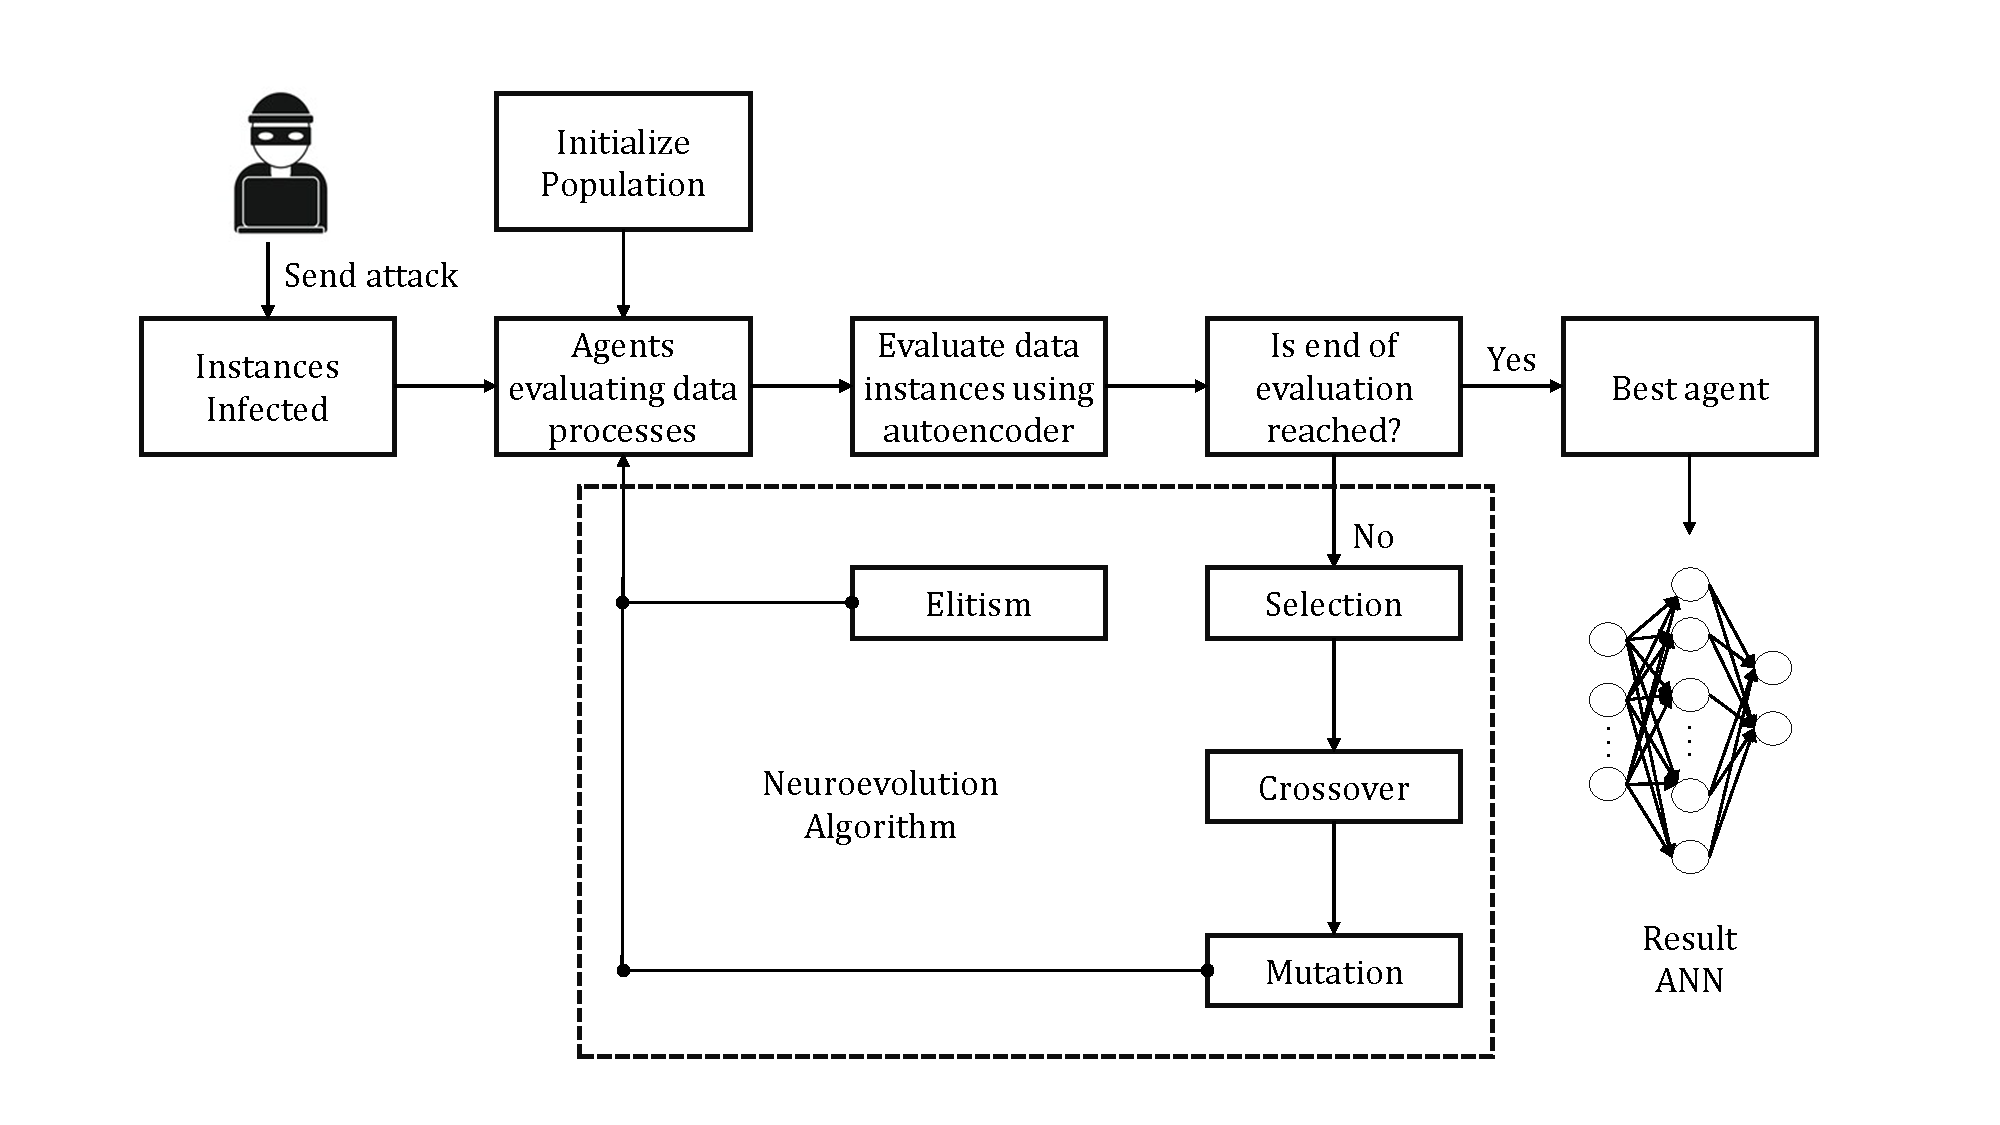
\includegraphics[scale=0.5]{figs/neuroevolution/diag_neuroevolution.pdf}
\vspace{-0.5cm}
\caption{Neuroevolution algorithm flow.}
\label{fig:diagneuroevolution}
\end{figure*}




\section{Experiments and Results}
In this section, we present the results of the experiments carried out following the proposed algorithms in the previous sections. 

%\subsection{Experiments Setup Network}


\subsection{Feature selection}

Due to the high dimensionality of the dataset, it is necessary to discard certain features in order to improve the perfomance of the model. Firstly, to reduce the number of variables, a previous study of each variable was made, comparing the results between the different states of the machine. The first variables to delete were those are not affected in either state of the virtual instance. In this way, 26 of the 97 initial variables that only accounted for computational load when training the neural network were eliminated, in addition to overtraining. \\

It is well known that multicollinearity in data considerably reduces the predictive power of many machine learning models. Despite the fact that an autoencoder is not a linear model, it is convenient to reduce this high dimensionality of the data in any case and an important measure to do so, is through correlation. \\



\begin{table*}[h!]
\begin{tabular}{ccc}
\hline
Variable 1 & Variable 2 & Correlación \\ \hline
load 15 & load norm 15 & 1.0\\ 
load norm 1 & load 1 & 1.0\\ 
memory used bytes & memory free & 1.0\\ 
memory actual used bytes & memory actual free & 1.0\\ 
load norm 5 & load 5 & 1.0\\ 
filesystem free & filesystem available & 0.99\\ 
memory used bytes & memory used pct & 0.991\\ 
memory free & memory used pct & 0.99\\ 
memory actual free & memory actual used pct & 0.99\\ 
memory actual used bytes & memory actual used pct & 0.99\\ 
entropy available bits & entropy pct & 0.99\\ 
core idle pct & cpu idle pct & 0.99\\ 
core system pct & cpu system pct & 0.99\\ 
core user pct & cpu user pct & 0.99\\ 
core nice pct & cpu nice pct & 0.99\\ 
cpu iowait pct & core iowait pct & 0.99\\ 
diskio io time & diskio write count & 0.99\\ 
process summary sleeping & process summary total & 0.98\\ 
diskio write bytes & diskio io time & 0.98\\ 
cpu total pct & core idle pct & 0.98\\ 
cpu total pct & cpu idle pct & 0.98\\ 
fsstat total size used & fsstat total size free & 0.987\\ 
diskio io time & diskio write time & 0.98\\ 
fsstat total size used & filesystem used bytes & 0.97\\ 
diskio write bytes & diskio write count & 0.96\\ 
filesystem used bytes & filesystem used pct & 0.96\\ 
fsstat total size free & filesystem used pct & 0.96\\ 
diskio write count & diskio write time & 0.95\\ 
fsstat total size free & filesystem used bytes & 0.94\\ 
diskio iostat write request per sec & diskio iostat busy & 0.94\\ 
filesystem free & filesystem free files & 0.92\\ 
filesystem available & filesystem free files & 0.92\\ 
diskio iostat await & diskio iostat write await & 0.92\\ 
socket summary all count & socket summary udp all count & 0.91\\ 
socket summary tcp all established & socket summary tcp all count & 0.917\\ 
diskio iostat queue avg size & diskio iostat busy & 0.90\\ \hline

\end{tabular}
\label{tabla:sencilla}
\caption{Pearson correlation ($\rho$) table for variables with correlation coefficient $\rho>0.90$.}
\end{table*}

In this way, it was first established that variables were strongly related to each other (a correlation coefficient higher than 0.7) and once the relationships were obtained, a study was carried out on the variables themselves, that is, the definition of the variables themselves. Thus, if two variables explained the same information, one of them would be discarded. It was also tried to have at least one representative variable for each module in order to have more complete information on the system. After this study, a total of 58 out of 97 variables were discarded.


\subsection{Results}


The results show that it is possible to determine the state of a instance using autoencoders and also detect malicious processes that affect the normal behaviour of a computer. So the results are presented in two steps: anomaly detection resultas and evolutionary algorithms for neural networks.


\subsubsection{Autoencoder model results}\label{results_autoencoder}

The autoencoder model was trained with only the healthy state of the data using the stochastic gradient descent algorithm with 60 epochs. The mean square error was monitored during the training process, the results are shown in Figure \ref{fig:autoencoder_variable_selected}.



\begin{figure}[h!]
\centering
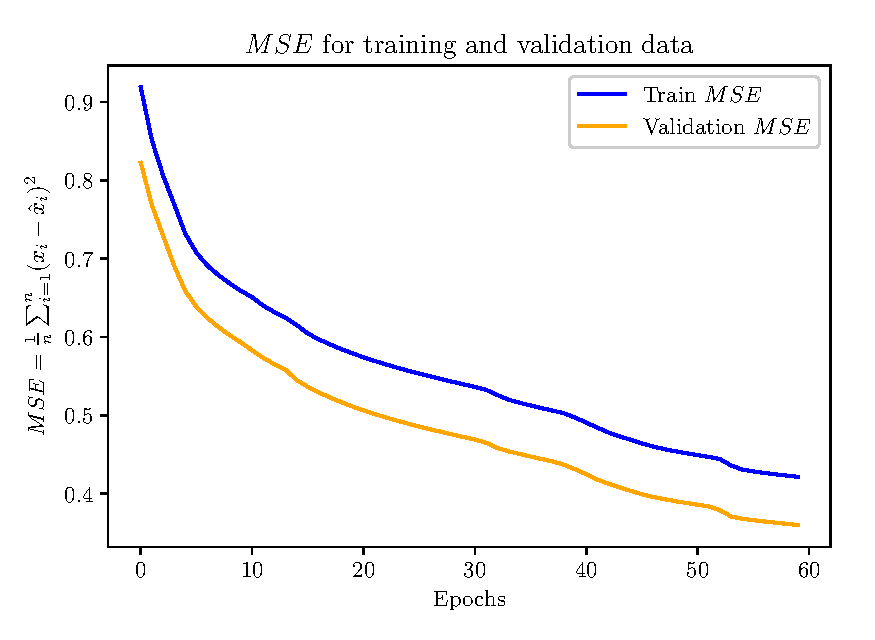
\includegraphics[scale=0.56]{figs/autoencoder/final_autoencoder.eps}
\caption{Nº epochs vs. $MSE$. Mean square error for a trained (Train) and validated (Validation) data for the autoencoder neural network with data from healthy machines after feature selection.}
\label{fig:autoencoder_variable_selected}
\end{figure}

After training the model, it is necessary to determine the decision threshold from which the state of the machine is considered an anomaly, for this, the Algorithm \ref{obtener_umbral} was used, giving a threshold $\alpha\approx 1.1945\ldots$, the closer value to this the state of the instance is, the greater the consideration will be as a healthy state of the instance. Therefore the agents of the evolutionary algorithm should eliminate the process that is affecting the instance and will be selected as the best ``parents'' those that after killing the process, lead to the state of the instance at values close to this $\alpha$ value. The resuls are shown in Figure \ref{fig:reconstuction_LB}.

\begin{figure}[h!]
\centering
\includegraphics[scale=0.56]{figs/autoencoder/reconstruccion_error_LB.eps}
\caption{Threshold decision from the mean square error (MSE). The red line represents the threshold decision $\alpha\approx1.1945\ldots$ to classify the anomaly.}
\label{fig:reconstuction_LB}
\end{figure}

With this decision threshold, a confusion matrix is obtained in order to try using the autoencoder also as a classifier. The results are shown in Table \ref{confusion_matrix}. \\

\begin{table}[h!]
\centering
\begin{tabular}{llll}
                                                &                                 & \multicolumn{2}{c}{Real}                                       \\ \cline{3-4} 
                                                & \multicolumn{1}{l|}{}           & \multicolumn{1}{l|}{L. Bomb} & \multicolumn{1}{l|}{Healthy} \\ \cline{2-4} 
\multicolumn{1}{c|}{Predicted} & \multicolumn{1}{l|}{L. Bomb} & \multicolumn{1}{l|}{1629}       & \multicolumn{1}{l|}{174}     \\ \cline{2-4} 
\multicolumn{1}{c|}{}                           & \multicolumn{1}{l|}{Healthy}    & \multicolumn{1}{l|}{135}        & \multicolumn{1}{l|}{5457}    \\ \cline{2-4} 
\end{tabular}
\caption{Confusion matrix build from threshold decision $\alpha$. The classification is done following if $MSE>\alpha\implies$ infected instance.}
\label{confusion_matrix}
\end{table}

Then, a 10-fold cross validation is done and finally we get the following performance measures (mean of the 10-fold results), which usually are taken into account to determine the goodness of fit.


\begin{alignat*}{3}
\hspace{-0.3cm} Accuracy  &= \hspace{0.9cm}\frac{\text{Correctly classified}}{\text{Total of samples}}           &&=&\text{ }& 0.9632 \\
\hspace{-0.3cm} Precision &=\frac{\text{Correctly classified as infected}}{\text{Samples predicted as infected}} &&=&\text{ }& 0.9335\\
\hspace{-0.3cm} Recall    &=\frac{\text{Correctly classified as infected}}{\text{Samples actually are infected}} &&=&\text{ }& 0.9136\\
\end{alignat*}

These results show that our autoencoder model can classify states of the virtual machines using anomaly detection and being trained just with one kind of data (healthy state).


\subsubsection{Neuroevolution results}

In this section we will present the most important results of this paper. We will see how a neural network trained with a hybrid machine learning algorithm with evolutionary algorithms is able to reduce the effect of these attacks on virtual instances. \\


\begin{figure*}[h!]
\begin{subfigure}{.49\linewidth}
\centering
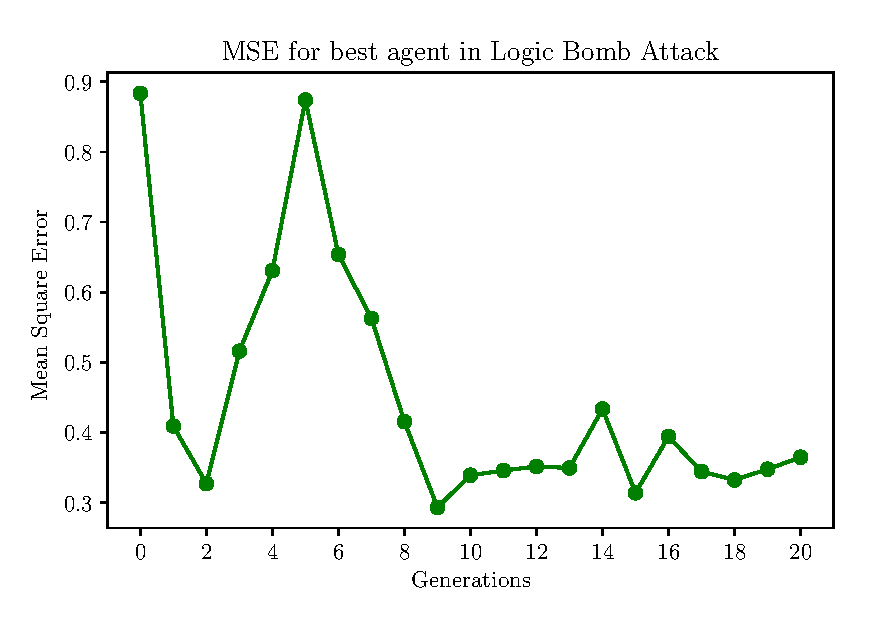
\includegraphics[width=\linewidth]{figs/results/reward_best_agent_final.eps}
\end{subfigure}
\begin{subfigure}{.49\linewidth}
\centering
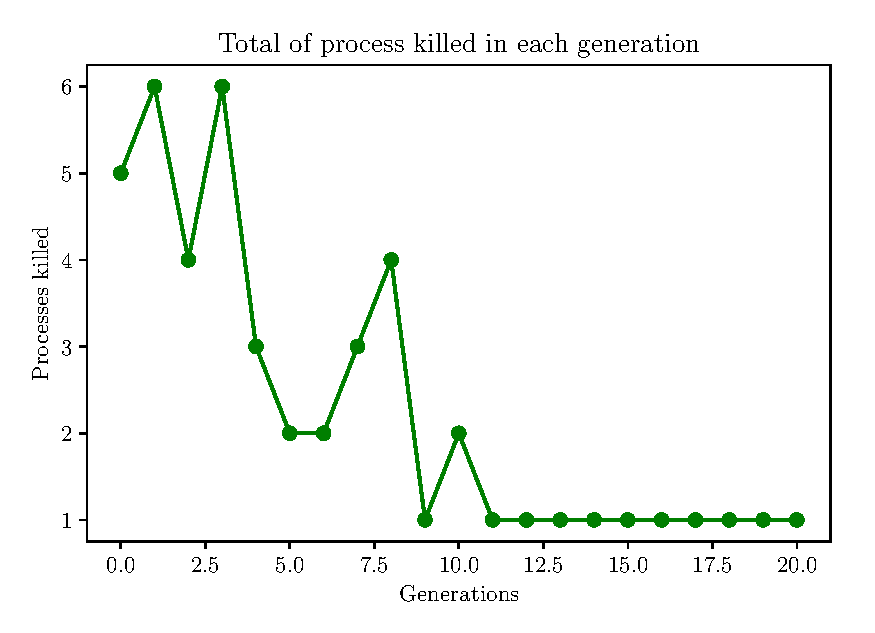
\includegraphics[width=\linewidth]{figs/results/number_process_final_top_agent.eps}
\end{subfigure}
\caption{(Left) Rewards (MSE) for the best agent in each generation using an algorithm to evolve neural networks and (right) total processes that are killed in each generation evolving neural networks using as fitness function the MSE given by the autoencoder (Equation \ref{fitness}).}
\label{fig:reward_top_agent}
\end{figure*}

From the generation 10, it is appreciated (Figure \ref{fig:reward_top_agent}) that the best agent is able to reduce the mean squared error at the output of the autoencoder. For this, the best agent kills the processes that are considered by it as malicious, so the objective is not only kill all processes but kill the specific process who is affecting the virtual instance, so as we can se in Figure \ref{fig:reward_top_agent} the best agent reduce the number of processes that it pretends to kill until finally kill just the malicious process.\\


\section{Conclusions}

In this paper we have shown other way to reduce the effect of cyber attacks and as well as another application that has the neuroevolution algorithms who has never applied in cyber security. We have confimed the results of other researchers \cite{autoencoderdos} using an autoencoder to classify cyber attacks, although in our case we have used other methodology and other cyber attack. The autoencoders can give you a measure of how close to a healthy state a virtual instance is, this allow us to combine this measure with a neuroevolution algorithm to select the best agents, giving as a result an ingenious hybrid algorithm able to detect malicious processes that are being running in our shell. 


\appendix
\section{Appendix: Description of each variable}\label{appx_variables}

\subsection{Central Processing Unit (CPU) Features}

\textbf{cpu\_cores:} The number of CPU cores present on the host. The non-normalized percentages will have a maximum value of 100\% $\cdot$ cores. The normalized percentages already take this value into account and have a maximum value of 100\%.\\

\textbf{cpu\_user\_pct:} The percentage of CPU time spent in user space. On multi-core systems, you can have percentages that are greater than 100\%. For example, if 3 cores are at 60\% use, then the system.cpu.user.pct will be 180\%.\\

\textbf{cpu\_system\_pct:} The percentage of CPU time spent in kernel space.\\

\textbf{cpu\_nice\_pct:} The percentage of CPU time spent on low-priority processes.\\

\textbf{cpu\_idle\_pct:} The percentage of CPU time spent idle.\\

\textbf{cpu\_iowait\_pct:} The percentage of CPU time spent in wait (on disk).\\

\textbf{cpu\_irq\_pct:} The percentage of CPU time spent servicing and handling hardware interrupts.\\

\textbf{cpu\_softirq\_pct:} The percentage of CPU time spent servicing and handling software interrupts.\\

\textbf{cpu\_steal\_pct:} The percentage of CPU time spent in involuntary wait by the virtual CPU while the hypervisor was servicing another processor.\\

\textbf{cpu\_total\_pct:} The percentage of CPU time spent in states other than Idle and IOWait.\\


\subsection{Core features}

\textbf{core\_user\_pct:} The percentage of CPU time spent in user space.\\

\textbf{core\_system\_pct:} The percentage of CPU time spent in kernel space.\\

\textbf{core\_nice\_pct:} The percentage of CPU time spent on low-priority processes.\\

\textbf{core\_idle\_pct:} The percentage of CPU time spent idle..\\

\textbf{core\_iowait\_pct:} The percentage of CPU time spent in wait (on disk).\\

\textbf{core\_irq\_pct:} The percentage of CPU time spent servicing and handling hardware interrupts.\\

\textbf{core\_softirq\_pct:}The percentage of CPU time spent servicing and handling software interrupts.\\

\textbf{core\_steal\_pct:}  The percentage of CPU time spent in involuntary wait by the virtual CPU while the hypervisor was servicing another processor. Available only on Unix.


\subsection{Disk Input/Output (Disk I/O) features}

\textbf{diskio\_read\_count:} The total number of reads completed successfully.\\

\textbf{diskio\_write\_count:} The total number of writes completed successfully.\\

\textbf{diskio\_read\_bytes:} The total number of bytes read successfully. On Linux this is the number of sectors read multiplied by an assumed sector size of 512.\\

\textbf{diskio\_write\_bytes:} The total number of bytes written successfully. On Linux this is the number of sectors written multiplied by an assumed sector size of 512.\\

\textbf{diskio\_read\_time:} The total number of milliseconds spent by all reads.\\

\textbf{diskio\_write\_time:} The total number of milliseconds spent by all writes.\\

\textbf{diskio\_io\_time:} The total number of of milliseconds spent doing I/Os.\\

\textbf{diskio\_iostat\_read\_request\_merges\_per\_sec:} The number of read requests merged per second that were queued to the device.\\

\textbf{diskio\_iostat\_write\_request\_merges\_per\_sec:} The number of write requests merged per second that were queued to the device.\\

\textbf{diskio\_iostat\_read\_request\_per\_sec:} The number of read requests that were issued to the device per second.\\

\textbf{diskio\_iostat\_wirte\_request\_per\_sec:} The number of write requests that were issued to the device per second.\\

\textbf{diskio\_iostat\_read\_per\_sec\_bytes:} The number of Bytes read from the device per second.\\

\textbf{diskio\_iostat\_read\_await:} The average time spent for read requests issued to the device to be served.\\

\textbf{diskio\_iostat\_write\_per\_sec\_bytes:}  The number of Bytes write from the device per second.\\

\textbf{diskio\_iostat\_write\_await:} The average time spent for write requests issued to the device to be served.\\

\textbf{diskio\_iostat\_request\_avg\_size:} The average size (in bytes) of the requests that were issued to the device.\\

\textbf{diskio\_iostat\_queue\_avg\_size:}The average queue length of the requests that were issued to the device.\\

\textbf{diskio\_iostat\_await:} The average time spent for requests issued to the device to be served.\\

\textbf{diskio\_iostat\_service\_time:} The average service time (in milliseconds) for I/O requests that were issued to the device.\\

\textbf{diskio\_iostat\_busy:} Percentage of CPU time during which I/O requests were issued to the device (bandwidth utilization for the device). Device saturation occurs when this value is close to 100\%.\\


\subsection{Entropy}

\textbf{entropy\_available\_bits:} The available bits of entropy.\\

\textbf{entropy\_pct:} The percentage of available entropy, relative to the pool size of 4096.\\



\subsection{Filesystem}

\textbf{filesystem\_available:} The disk space available to an unprivileged user in bytes.\\

\textbf{filesystem\_files:} The total number of file nodes in the file system.\\

\textbf{filesystem\_free:} The disk space available in bytes.\\

\textbf{filesystem\_free\_files:} The number of free file nodes in the file system.\\

\textbf{filesystem\_total:} The total disk space in bytes.\\

\textbf{filesytem\_used\_bytes:} The used disk space in bytes.\\

\textbf{filesystem\_used\_pct:} The percentage of used disk space.\\

\textbf{fsstat\_count:} Number of file systems found.\\

\textbf{fsstat\_total\_files:} Total number of files.\\

\textbf{fsstat\_total\_size\_free:} Total free space.\\

\textbf{fsstat\_total\_size\_used:} Total used space.\\

\textbf{fsstat\_total\_size\_total:} Total space (used plus free).\\

\subsection{Memory Swap}

\textbf{memory\_swap\_pct:} Total swap memory.\\

\textbf{memory\_swap\_used\_bytes:} Used swap memory in bytes.\\

\textbf{memory\_swap\_free:} Available swap memory.\\

\textbf{memory\_swap\_used\_pct:} The percentage of used swap memory.\\


\subsection{Memory hugepages}

\textbf{memory\_hugepages\_total:} Number of huge pages in the pool.\\

\textbf{memory\_hugepages\_used\_bytes:} Memory used in allocated huge pages in bytes.\\

\textbf{memory\_hugepages\_used\_pct:} Percentage of huge pages used.\\

\textbf{memory\_hugepages\_free:} Number of available huge pages in the pool.\\

\textbf{memory\_hugepages\_reserved:} Number of reserved but not allocated huge pages in the pool.\\

\textbf{memory\_hugepages\_surplus:} Number of overcommited huge pages.\\

\textbf{memory\_hugepages\_default\_size:} Default size for huge pages.




\subsection{Socket summary}

\textbf{socket\_summary\_all\_count:} All open connections.\\

\textbf{socket\_summary\_all\_listening:} All listening ports.\\

\textbf{socket\_summary\_tcp\_memory:} Memory used by  \textit{Transmission Control Protocol} (TCP) sockets in bytes, based on number of allocated pages and system page size. \\

\textbf{socket\_summary\_tcp\_all\_orphan:} A count of all orphaned tcp sockets.\\

\textbf{socket\_summary\_tcp\_all\_count:} All open TCP connections.\\

\textbf{socket\_summary\_tcp\_all\_listening:} All TCP listening ports.\\

\textbf{socket\_summary\_tcp\_all\_established:} Number of established TCP connections.\\

\textbf{socket\_summary\_tcp\_all\_close\_wait:} Number of TCP connections in \textit{close\_wait} state.\\

\textbf{socket\_summary\_tcp\_all\_time\_wait:} Number of TCP connections in \textit{time\_wait} state.\\

\textbf{socket\_summary\_udp\_memory:} Memory used by UDP sockets in bytes, based on number of allocated pages and system page size.\\

\textbf{socket\_summary\_udp\_all\_count:} All open UDP connections.\\


%================== Appendix II =====================% 

\section{Appendix: Description of each variable for the agents.}


\subsubsection{File descriptors}

\textbf{process\_fd\_limit\_hard:} limit hard on the number of file descriptors opened by the process. The hard limit can only be increased by root.\\

\textbf{process\_fd\_limit\_soft:} limit soft on the number of file descriptors opened by the process. The process can change the limit soft at any time.\\

\textbf{process\_fd\_open:} the number of file descriptors opened by the process.\\


\subsubsection{Central Processing Unit (CPU)}

\textbf{process\_cpu\_total\_norm\_pct:} Percentage of CPU time that the process consumes since the last event. This value is normalized by the number of CPU cores and ranges from 0\% to 100\%.\\

\subsubsection{Memory}

\textbf{process\_memory\_size:} The total in bytes of virtual memory that the process has.\\

\textbf{process\_memory\_rss\_bytes:} The Resident Set Size (RSS) in bytes. The proportion of memory used by a process that is held in main memory (RAM), that is, the memory that the process occupied in main memory or RAM.\\

\textbf{process\_memory\_share:} the shared memory in bytes that the process uses.\\

\subsubsection{Temporal features}

\textbf{process\_cpu\_start\_time\_seconds:} The time (in seconds) since the process started.\\




























\subsection{Body of the text}
\begin{itemize}
\item The use of first persons (i.e., ``I'', ``we'', ``their'', possessives, etc.) should be avoided,
and can preferably be expressed by the passive voice or other ways. This also applies to the Abstract.
\item A research paper should be structured in terms of four parts, each of which may comprise of multiple sections:
\begin{itemize}
\item Part One is problem description/definition, and a literature review upon the state of the
art
\item Part Two is methodological formulation and/or theoretical development (fundamentals, principle and/or approach,
etc.)
\item Part Three is prototyping, case study or experiment;
\item Part Four is critical evaluation against related works, and the
conclusion.
\end{itemize}
\item A survey paper may skip Part Three, but should multiply Part Two and elaborate Parts One and Four.
\item An application paper may lightly touch Part Two but should elaborate Part Three, with Parts One and Four similar to the a
research paper.
\end{itemize}

In any article it is unnecessary to have an arrangement statement at the beginning (or end) of every \mbox{(sub-)} section.
Rather, a single overall arrangement statement about the whole paper can be made at the end of the Introduction section.


\section{Typographical style and layout}

\subsection{Type area}

The \texttt{iosart2c.cls} document class has been designed to produce
the right layout from your \LaTeX{} input. Authors are requested to
strictly follow these instructions. \emph{The provided class file
iosart2c must not be changed}.

The text output area is automatically set within an area 16.2 cm
horizontally and 21.5 cm vertically. Please do not use any
\LaTeX{} or \TeX{} commands that affect the layout or formatting of
your document (i.e. commands like \verb|\textheight|,
\verb|\textwidth|, etc.).

\subsection{Font}

The font type for running text (body text) is 10~point Times New Roman.
There is no need to code normal type (roman text). For literal text, please use
\texttt{type\-writer} (\verb|\texttt{}|)
or \textsf{sans serif} (\verb|\textsf{}|). \emph{Italic} (\verb|\emph{}|)
or \textbf{boldface} (\verb|\textbf{}|) should be used for emphasis.


\subsection{General layout}

Use single (1.0) line spacing throughout the document. For the main
body of the paper use the commands of the standard \LaTeX{}
``article'' class. You can add packages or declare new \LaTeX{}
functions if and only if there is no conflict between your packages
and the \texttt{iosart2c.cls}.

Always give a \verb|\label| where possible and use \verb|\ref| for cross-referencing.

Class option ``\texttt{onecolumn}'' should be used only if it is
necessary for the layout of your article:\hfill\break
\verb|\documentclass[onecolumn]{iosart2c}|.

Use class option ``\texttt{crcready}'' in order to remove the page numbers from your article.


\subsection{Title page}

Use sentence case for the title.

Use \verb|\thanks{}| command for footnotes in\break \verb|\title|,
\verb|\author| and \verb|\address| commands.

Do not use capitals for author's surname. Add ``and'' before the last
author. Do not add a period after the last keyword.


\subsection{(Sub-)section headings}

Use the standard \LaTeX{} commands for headings: \verb|\section|, \verb|\subsection|, \verb|\subsubsection|, \verb|\paragraph|.
Headings will be automatically numbered.

\subsection{Footnotes and endnotes}
Footnotes should only be used if absolutely essential.
In most cases it is possible to incorporate the information in the text.
If used, they should be kept as short as possible.
The footnotes are numbered automatically. If the footnotes take up more space than roughly 10\% of the type area,
list them as endnotes, before the References. Footnotes within the text should be coded with the command
\verb|\footnote{Text}|,
 endnotes with the command \verb|\endnote{Text}|.
The command \verb|\theendnotes| prints out the endnotes.
The additional package \texttt{endnotes} is required for the endnotes (\verb|\usepackage{endnotes}|).
If you do not have it in your \LaTeX{} environment,
see your system manager, or download them from http://www.ctan.org.



\subsection{References}

References should be collected at the end of your paper (environment
\verb|thebibliography|). References should be listed alphabetically in the style presented in the section \textbf{References} at the
end of these instructions. Use the command \verb|\cite| to refer to the entries in the bibliography so that your
accumulated list corresponds to the citations made in the text body.

\begin{figure}[t]
\leavevmode\fbox{\parbox[b][30mm][s]{30mm}{
\vfill\footnotesize Please include graphics in Encapsulated
PostScript (.eps) format\vfill}}
\caption{Figure caption.}
\end{figure}


\subsection{Figures}
\subsubsection{General remarks on figures}
The text should include references to all figures.
Refer to figures in the text as Figure 1, Figure 2, etc., \textbf{not} with the section number included,
e.g. Figure 2.3, etc. Do not use the words ``below'' or ``above'' when referring to the
figures.

Do not collect figures at the back of your article, but incorporate them in the text.

Position figures at the top or bottom of a page, near the paragraph in which the figure is first mentioned.
Figures should not have text wrapped alongside.

Each figure should have a self-explanatory caption. Place the figure caption \textit{below} the figure.

All figures coded with \verb|figure| and \verb|\caption| will be numbered automatically.

On maps and other figures where a scale is needed, use bar scales rather than numerical ones of the type 1:10,000.

%They will be numbered automatically.

\subsubsection{Quality of illustrations}
Use only Type I fonts for the lettering in illustrations. Do \textit{not} use illustrations taken from the Internet.
The resolution of images intended for viewing on a screen is not sufficient for the printed version of the journal.
If you are incorporating screen captures, keep in mind that the text may not be legible after reproduction
(using a screen capture tool, instead of the Print Screen option of PC's, might help to improve the
quality). Preferably the images should be enclosed as PostScript
files -- best as EPS data.


\begin{table*}[htb]
\caption{Table caption} \label{t1}
\begin{tabular}{ll d{1.3} d{1.3} d{1.3} d{1.3} d{1.3} d{1.3}}
\hline
Dataset&Models&\multicolumn{1}{l}{$\alpha_1$}&
\multicolumn{1}{l}{$\alpha_2$}&
\multicolumn{1}{l}{$\alpha_3$}&
\multicolumn{1}{l}{$\alpha_4$}&
\multicolumn{1}{l}{$\alpha_5$}&
\multicolumn{1}{l}{$\alpha_6$}\\
\hline
CSDS&Linear     &0.164&0.22&0.123&0.3&0.200&0.258\\
& Logistic      &0.189&0.155&0.157&0.201&0.154&0.144\\[6pt]
KCDS&Linear     &0.155&0.183&0.160&0.218&0.176&0.156\\
& Logistic      &0.187&0.125&0.151&0.184&0.187&0.125\\
\hline
\end{tabular}
\end{table*}



\begin{itemize}
\item Line art should have a minimum resolution of 600 dpi;  %, save as EPS or TIFF
\item  grayscales (incl photos) should have a minimum resolution of 300 dpi (no lettering), or 500 dpi (when there is lettering); %save as tiff
\item  do not save figures as JPEG, this format may lose information in the
process;
\item  do not use figures taken from the Internet, the resolution will be too low for
printing;
\item  do not use color in your figures if they are to be printed in black \& white, as this will reduce the print
quality (note that in software the default is often color, so you should change the
settings);
\item  for figures that should be printed in color, please send a CMYK encoded EPS.% or TIFF
\end{itemize}

\subsubsection{Color figures}
It is possible to have figures printed in color,
provided the cost of their reproduction is paid for by the author.
Please contact editorial@iospress.nl for a quotation if you wish to have figures printed in color.
See section \ref{s3.8.2} for the required file formats.

\subsection{Tables}

The text should include references to all tables.
Refer to tables in the text as Table 1, Table 2, etc., not with the section number included,
 e.g. Table 2.3, etc. Do not use the words ``below'' or ``above'' referring to the
 tables.

Position tables at the top or bottom of a page, near the paragraph in which the table is first mentioned.
Tables should not have text wrapped alongside.


Code your tables using \LaTeX{} environments \verb|table| and
\verb|tabular|. Each table should have a brief and self-explanatory caption that should be put above the
table. Do not use the period at the end of the table caption. If the table does not fit into one column it may be placed across both columns
using \verb-\begin{table*}-
so that it
appears at the top of a page.




All tables coded with \verb|table| and \verb|\caption| will be numbered automatically.

Column headings should be brief, but sufficiently explanatory.
Standard abbreviations of units of measurement should be added between parentheses.
Vertical lines should not be used to separate columns. Leave some extra space between the columns instead.
Any explanations essential to the understanding of the table should be given in footnotes at the bottom of the table.
SI units should be used, i.e., the units based on the metre, kilogramme, second, etc.

Tables should be presented in the form shown in
Table~\ref{t1}.  Their layout should be consistent
throughout.





\subsection{Equations}

Do not put in equation numbers, since this is taken care of
automatically. The equation numbers are always consecutive and are
printed in parentheses flush with the right-hand margin of the text and
level with the last line of the equation. For multi-line equations, use
the {\tt eqnarray} environment. Refer to equations in the text as Eq. (1), Eqs. (3) and (5).


\section{Fine tuning}
\subsection{Type area}
Check once more that all the text and illustrations are inside the type area and
that the type area is used to the maximum.

\subsection{Capitalization}
Use sentence case in the title and the headings.

\subsection{Page numbers and running headlines}
You do not need to include page numbers or running headlines. These elements will be added by the publisher.

\section{Submitting the paper}
Submit the following to the journal Editorial office, online submission form or Editor-in-Chief (whichever is applicable for the journal):

\begin{enumerate}
\item The main \LaTeX{} document as well as other required files (eps, etc.).
\item Identical high resolution PDF file with all fonts embedded. First produce a Postscript file from \LaTeX{}
with DVIPS version 5.56 or higher. The option "-M" (don't make fonts) should be indicated.
Use Adobe Acrobat Distiller and choose the job option Press-Optimized.) Please make sure you do not submit more than one version of any item.
\end{enumerate}

\section{Copyright}
Authors submitting a manuscript do so in the understanding that they have read and agreed to the terms of the IOS Press Author
Copyright Agreement posted in the `Authors Corner' on www.iospress.nl.

\subsection{Quoting from other publications}
An author, when quoting from someone else's work or when considering reproducing figures or tables from a book or journal article,
 should make sure that he/she is not infringing a copyright. Although in general an author may quote from other published works,
 he should obtain permission from the holder of the copyright if he wishes to make substantial extracts or to reproduce tables,
  plates or other figures. If the copyright holder is not the author of the quoted or reproduced material, it is recommended
  that the permission of the author should also be sought. Material in unpublished letters and manuscripts is also protected
  and must not be published unless permission has been obtained. Submission of a paper will be interpreted as a statement that
the author has obtained all the necessary permission. A suitable acknowledgement of any borrowed material must always be made.

\section{How to order reprints, a pdf file, journals, or IOS Press
books}
The corresponding author of a contribution to the journal is entitled to receive 1 copy of the journal free of charge, unless otherwise stated. Free copies will not be provided for conference proceedings and abstract issues. An order form for reprints,
additional journal copies or a pdf file will be provided along with the pdf proof.
If you wish to order reprints of an earlier published article, please contact the publisher for a quotation at IOS Press, Fax:
+31 20 6870039. E-mail:\break editorial@iospress.nl.
An author is entitled to 25\% discount on IOS Press books.\vadjust{\vfill\eject}

\begin{thebibliography}{0}


\end{thebibliography}


\end{document}
